\documentclass[conference]{IEEEtran}

\usepackage[utf8]{inputenc}
\usepackage[T1]{fontenc}
\usepackage{cite}
\usepackage{amsmath,amssymb}
\usepackage{graphicx}
\usepackage{booktabs}
\usepackage{url}
\usepackage{hyperref}
\usepackage{xcolor}
\usepackage{multirow}
\usepackage{subcaption}
\usepackage{tikz}
\usetikzlibrary{shapes.geometric, arrows.meta, positioning, fit, backgrounds}

\begin{document}

\title{SWE-Bench 5G: A Benchmark for Evaluating AI Coding Agents on 5G Core Network Engineering Tasks}

\author{
\IEEEauthorblockN{Anonymous Author(s)}
}

\maketitle

\begin{abstract}
AI coding agents have demonstrated strong performance on general-purpose software benchmarks such as SWE-Bench and BeyondSWE, yet no existing benchmark evaluates their capabilities on telecommunications software. We introduce SWE-Bench~5G, the first benchmark for evaluating AI coding agents on real bug-fixing tasks drawn from the free5GC open-source 5G core network. The benchmark comprises 210 validated task instances spanning 9 Network Functions (NFs), each packaged as a self-contained Docker environment with automated tests. We evaluate four LLMs under two agent paradigms, single-turn and multi-turn with iterative feedback, and find that agentic capabilities, rather than model intelligence alone, constitute the primary bottleneck: all models correctly diagnose bugs at rates exceeding 80\%, but only multi-turn agents successfully apply patches. We further investigate specification-as-skill injection by adapting the methodology of SWE-Skills-Bench to the 3GPP domain and find that protocol specification excerpts yield a 10\% overall resolve rate improvement, concentrated on specification-dependent bugs while providing no benefit for generic null-check bugs. The benchmark, evaluation harness, and dataset are publicly available at \url{https://huggingface.co/datasets/tenderzada/SWEBench5G}.
\end{abstract}

% ============================================================
\section{Introduction}
% ============================================================

Large language models (LLMs) have enabled a new class of AI coding agents that autonomously navigate codebases, diagnose bugs, and generate patches~\cite{jimenez2024swebench}. Benchmarks such as SWE-Bench~\cite{jimenez2024swebench}, BeyondSWE~\cite{shi2025beyondswe}, and SWE-Skills-Bench~\cite{han2025sweskills} have driven rapid progress, but they target general-purpose software, primarily Python, and leave a critical question open: can coding agents operate effectively in specification-driven vertical domains?

The 5G core network (5GC) presents a compelling test case. Defined by hundreds of 3GPP Technical Specifications (TS), 5GC implementations translate precise protocol semantics into production code decomposed across multiple Network Functions (NFs). Bugs in this domain differ fundamentally from those in typical open-source projects. First, correctness is defined by normative protocol text, not just passing tests. Second, distributed microservice architectures span multiple NFs communicating via HTTP/2 and PFCP. Third, protocol state machines impose complex multi-step procedures for registration, session management, and mobility.

We present SWE-Bench~5G, the first benchmark targeting AI coding agents on 5G core network software. Drawing from free5GC~\cite{free5gc}, an open-source Go implementation of the 3GPP 5GC, we construct 210 validated task instances spanning 9~NFs from over 500 candidates mined across 20 repositories. Following BeyondSWE~\cite{shi2025beyondswe}, each instance provides a reproducible Docker environment with fail-to-pass tests. Our contributions are threefold:

\begin{enumerate}
\item A benchmark framework mapping real 5G bugs to the SWE-Bench task format, with a dual test strategy designed for specification-driven code where standard unit testing is infeasible.
\item An evaluation of four LLMs under single-turn and multi-turn agent paradigms, revealing that agentic iteration, not domain knowledge, is the primary bottleneck.
\item A specification-as-skill A/B experiment adapting the methodology of SWE-Skills-Bench~\cite{han2025sweskills} to the 3GPP domain, demonstrating that specification utility depends on bug type.
\end{enumerate}

% ============================================================
\section{Related Work}
% ============================================================

\subsection{Software Engineering Benchmarks}

The evaluation of AI coding agents has evolved through several generations of benchmarks. SWE-Bench~\cite{jimenez2024swebench} pioneered this direction by drawing 2,294 task instances from 12 popular Python repositories on GitHub. Each instance pairs an issue description with a fail-to-pass test, enabling automated binary evaluation. The benchmark revealed that even frontier models initially achieved single-digit resolve rates, catalyzing a wave of agent architecture research.

Subsequent work expanded this paradigm along multiple axes. SWE-Bench Lite~\cite{jimenez2024swebench} selected a 300-instance subset for faster iteration. SWE-Bench Verified introduced human validation to remove ambiguous or under-specified instances. SWE-Bench Multimodal~\cite{yang2024swebenchmm} extended evaluation to visual software domains, requiring agents to process screenshots and UI specifications alongside code.

SWE-Bench Mobile~\cite{yao2025swebenchmobile} moved beyond Python to evaluate agents on a 500K-line iOS codebase in Swift and Objective-C. It introduced diff-based intent tests that verify patch correctness through structural source code inspection rather than runtime execution. This approach addresses the challenge of testing functions with complex runtime dependencies. We adapt this strategy for 5G NF functions that require SCTP connections, MongoDB contexts, or inter-NF signaling that cannot be easily mocked.

BeyondSWE~\cite{shi2025beyondswe} broadened the resolution scope to include cross-repository reasoning, domain-specific problem solving, and dependency-driven migrations, packaging each of its 500 instances in a Docker image for full reproducibility. By isolating each task in a container, BeyondSWE eliminated environment variability as a confounding factor. We adopt the same containerized design for SWE-Bench~5G.

\subsection{Skill Injection and Domain Knowledge}

A complementary research direction investigates whether external knowledge can improve agent performance. SWE-Skills-Bench~\cite{han2025sweskills} formalized this question by defining 49 programming skills and evaluating their injection into coding agents. Their central finding is that 80\% of skills provide zero improvement to resolve rates, with utility depending on domain match, abstraction level, and context compatibility. Skills that are too abstract (general coding guidelines) or too specific (API documentation for unrelated libraries) fail to help. Only skills that closely match the task domain and provide actionable, concrete guidance show positive effects.

This finding motivates our investigation of 3GPP specifications as skill documents. Unlike generic coding guidelines, 3GPP Technical Specifications define the authoritative ground truth for correct 5GC behavior and may therefore represent a category of high-utility, domain-matched skill.

\subsection{Gap: Telecommunications Software}

Despite the growing diversity of benchmarks, all existing work targets general-purpose software. No benchmark evaluates agents on protocol-specified, distributed telecommunications systems. The 5G domain introduces unique challenges: specification-driven correctness criteria, distributed NF coordination, and domain knowledge that is underrepresented in LLM training data relative to web development or data science.

% ============================================================
\section{Benchmark Design}
% ============================================================

\subsection{Overview}

Fig.~\ref{fig:overview} illustrates the SWE-Bench~5G evaluation pipeline. In Phase~1, an AI agent receives an issue description and the NF source code inside a Docker container, optionally augmented with a 3GPP specification excerpt, and produces a patch. In Phase~2, the patch is applied in a fresh container and validated against the test suite.

% ======== DRAWING PROMPT FOR FIG 1 (Gemini API) ========
% Prompt for Gemini image generation:
%
% Draw a two-phase system architecture diagram for an AI coding agent evaluation pipeline,
% styled for an IEEE academic paper (clean, professional, blue color scheme).
%
% Phase 1 (left side, light blue background, labeled "Phase 1: Agent Coding"):
% - A box "Issue / Problem Statement" (orange/tan) with an arrow pointing right to
% - A central box "AI Agent (LLM)" (yellow/light)
% - Above the agent, a dashed-border box "3GPP Spec (Optional)" with a dashed arrow down to the agent
% - Below the agent, a box "Docker Container (NF Source Code)" with bidirectional arrows to the agent
%   (labeled "Read Code" going up, "Edit Code" going down)
% - An arrow from the agent pointing right to a box "Proposed Patch"
%
% Phase 2 (right side, light green background, labeled "Phase 2: Rigorous Evaluation"):
% - "Proposed Patch" arrow pointing right to "Fresh Docker Container (Clean Env)"
% - Arrow down to "Apply Patch"
% - Arrow down to "Run Test Suite (P2P and F2P)"
% - Arrow down to "Verified Result" (with a checkmark icon)
%
% Style: rounded rectangles, clean sans-serif font, no 3D effects, thin borders,
% arrows are solid blue with arrowheads. The dashed arrow for optional spec uses gray dashed line.
% Background colors: Phase 1 = light blue (#E8F0FE), Phase 2 = light green (#E8F5E9).
% Overall white background. No drop shadows.
% Similar to the BeyondSWE/SearchSWE architecture diagram style.
% ======== END DRAWING PROMPT ========

\begin{figure}[t]
\centering
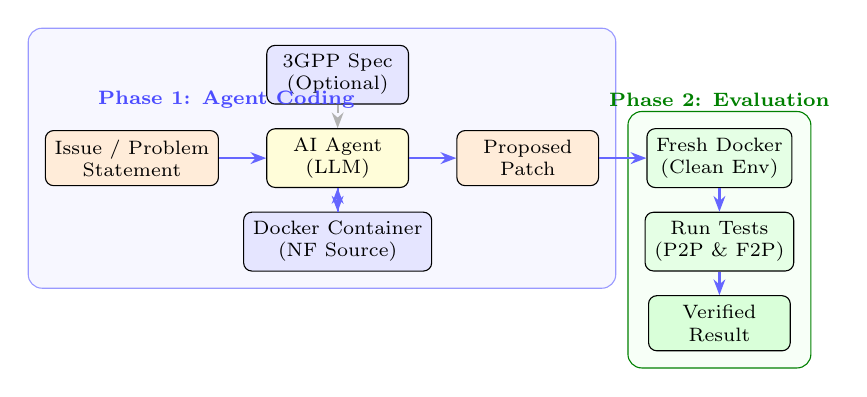
\begin{tikzpicture}[
    node distance=0.4cm and 0.3cm,
    box/.style={draw, rounded corners=3pt, minimum height=0.7cm, minimum width=1.8cm, font=\scriptsize, align=center, fill=#1},
    box/.default=blue!8,
    arrow/.style={-{Stealth[length=2mm]}, thick, draw=blue!60},
    dasharrow/.style={-{Stealth[length=2mm]}, thick, draw=gray!60, dashed},
    label/.style={font=\scriptsize\bfseries, text=blue!70},
    phase/.style={draw=blue!40, rounded corners=5pt, inner sep=6pt, fill=blue!3},
    phase2/.style={draw=green!50!black, rounded corners=5pt, inner sep=6pt, fill=green!3},
]
\node[box=orange!15] (issue) {Issue / Problem\\Statement};
\node[box=yellow!15, right=0.6cm of issue] (agent) {AI Agent\\(LLM)};
\node[box=blue!10, above=0.3cm of agent] (spec) {3GPP Spec\\(Optional)};
\node[box=blue!10, below=0.3cm of agent] (docker1) {Docker Container\\(NF Source)};
\node[box=orange!15, right=0.6cm of agent] (patch) {Proposed\\Patch};
\node[box=green!10, right=0.6cm of patch] (docker2) {Fresh Docker\\(Clean Env)};
\node[box=green!10, below=0.3cm of docker2] (test) {Run Tests\\(P2P \& F2P)};
\node[box=green!15, below=0.3cm of test] (result) {Verified\\Result};
\draw[arrow] (issue) -- (agent);
\draw[dasharrow] (spec) -- (agent);
\draw[arrow] (agent) -- (docker1);
\draw[arrow] (docker1) -- (agent);
\draw[arrow] (agent) -- (patch);
\draw[arrow] (patch) -- (docker2);
\draw[arrow] (docker2) -- (test);
\draw[arrow] (test) -- (result);
\node[label, above=0.15cm of issue, xshift=1.2cm] {Phase 1: Agent Coding};
\node[label, above=0.15cm of docker2, xshift=0.0cm, text=green!50!black] {Phase 2: Evaluation};
\begin{scope}[on background layer]
\node[phase, fit=(issue)(agent)(spec)(docker1)(patch)] {};
\node[phase2, fit=(docker2)(test)(result)] {};
\end{scope}
\end{tikzpicture}
\caption{SWE-Bench 5G evaluation pipeline. In Phase~1 the agent reads the issue and NF source code, optionally augmented with a 3GPP specification excerpt, and produces a patch. In Phase~2 the patch is applied in a fresh container and validated against pass-to-pass (P2P) and fail-to-pass (F2P) tests.}
\label{fig:overview}
\end{figure}

\subsection{Task Formulation}

Each task instance is a tuple $\mathcal{T} = (I, O, E)$ where $I$ is the input comprising a problem statement with optional 3GPP references and the NF source at the buggy commit, $O$ is the expected output in the form of a unified diff patch, and $E$ is the evaluation consisting of \texttt{PASS\_TO\_PASS} and \texttt{FAIL\_TO\_PASS} test suites. An instance is resolved if and only if all F2P tests pass and all P2P tests remain passing after applying the patch.

\subsection{Dual Test Strategy}

Many 5G NF functions cannot be unit-tested directly due to complex runtime dependencies such as SCTP connections, MongoDB sessions, and inter-NF signaling. We therefore employ two complementary strategies.

Strategy~A (Direct Call) applies when the buggy function accepts simple arguments. We call it directly with crash-triggering inputs and use Go's \texttt{defer/recover} mechanism to detect panics. This strategy is used for 68 of 210 instances.

Strategy~B (Diff-Based Intent), inspired by SWE-Bench Mobile~\cite{yao2025swebenchmobile}, verifies that the source code contains the expected fix pattern, for example checking that a nil guard exists before a pointer dereference. This forces agents to modify the source code without constructing complex mock objects. Strategy~B is used for 142 of 210 instances.

\subsection{Dataset Construction}

Our automated pipeline operates in five stages. First, we mine 20 free5GC sub-repositories via the GitHub API, collecting closed issues with linked merged pull requests and filtering by bug-fix keywords. This yields over 500 candidates. Second, quality filtering retains candidates with clear issue descriptions, source-modifying PRs, and bugs reproducible without external hardware. Third, we identify the parent (buggy) and fix commits for each candidate. Fourth, we construct fail-to-pass tests using Strategy~A or~B depending on function testability. Fifth, a batch validation script builds Docker images and runs three-step checks: existing tests pass at the parent commit, fail-to-pass tests fail at the parent commit, and all tests pass after applying the ground-truth fix. Only instances passing all checks are included.

Table~\ref{tab:dataset} summarizes the resulting dataset.

\begin{table}[t]
\centering
\caption{SWE-Bench 5G dataset statistics.}
\label{tab:dataset}
\begin{tabular}{@{}ll@{}}
\toprule
Attribute & Value \\
\midrule
Validated instances  & 210 \\
Source project       & free5GC (Go, Apache-2.0) \\
NFs covered          & 9 (AMF, SMF, PCF, UDM, UDR, NRF, \\
                     & \quad NSSF, AUSF, N3IWF) \\
Bug types            & nil pointer (89), crash/panic (42), \\
                     & \quad missing validation (35), logic error (27), \\
                     & \quad concurrency (17) \\
Difficulty           & Easy 126, Medium 62, Hard 22 \\
Test strategies      & 68 Direct Call (A) + 142 Diff-Based (B) \\
Avg. tests/instance  & 3.4 \\
3GPP specs referenced & 14 Technical Specifications \\
Candidate pool       & 500+ (from 20 repositories) \\
Docker base image    & \texttt{golang:1.25-bookworm} \\
\bottomrule
\end{tabular}
\end{table}

\subsection{NF Coverage}

Table~\ref{tab:nf} shows the distribution of instances across Network Functions. AMF and SMF contribute the most instances due to their larger codebases and higher issue volumes, while control-plane functions such as AUSF and NSSF have fewer instances reflecting their simpler implementations.

\begin{table}[t]
\centering
\caption{Instance distribution across Network Functions.}
\label{tab:nf}
\begin{tabular}{@{}llc@{}}
\toprule
NF & Role & Instances \\
\midrule
AMF  & Access and Mobility Management & 52 \\
SMF  & Session Management             & 41 \\
PCF  & Policy Control                 & 28 \\
UDM  & Unified Data Management        & 24 \\
UDR  & Unified Data Repository        & 22 \\
NRF  & NF Repository and Discovery    & 18 \\
NSSF & Network Slice Selection        & 11 \\
AUSF & Authentication Server          & 8  \\
N3IWF & Non-3GPP Interworking         & 6  \\
\bottomrule
\end{tabular}
\end{table}

% ============================================================
\section{Experimental Setup}
% ============================================================

\subsection{Agent Paradigms}

We evaluate two agent paradigms. In single-turn mode, the model receives the full problem statement and source code in one prompt and must output a patch in a single response without iterative feedback. In multi-turn mode, the agent operates in a loop of up to $K$ turns: generate patch, apply, compile, run tests, and if the tests fail, feed the error message back to the model for revision. We set $K{=}5$ in our experiments.

\subsection{Models}

We evaluate four LLMs selected for diversity across providers, as shown in Table~\ref{tab:models}. All models are accessed via standard OpenAI-compatible APIs.

\begin{table}[t]
\centering
\caption{Models evaluated in our experiments.}
\label{tab:models}
\begin{tabular}{@{}llll@{}}
\toprule
Model & Provider & API & Paradigm \\
\midrule
Qwen3.5-Flash   & Alibaba   & DashScope  & Single / Multi \\
Kimi-128k        & Moonshot  & Moonshot   & Multi \\
Claude Sonnet 4  & Anthropic & OpenRouter & Multi \\
GPT-4.1          & OpenAI    & OpenRouter & Multi \\
\bottomrule
\end{tabular}
\end{table}

\subsection{Specification-as-Skill Protocol}

Adapting the paired evaluation methodology of SWE-Skills-Bench~\cite{han2025sweskills}, we evaluate whether injecting 3GPP specification excerpts improves resolve rates. For each instance, a curated excerpt from the relevant Technical Specification is prepared, containing the applicable clause, field optionality rules, and a key implication paragraph linking the specification to the bug. Excerpts average 350 tokens.

We define two conditions: Condition~A ($-$spec) provides only the problem statement and source code, while Condition~B ($+$spec) additionally appends the 3GPP excerpt. Both conditions use identical Docker images, test suites, and evaluation criteria. We evaluate the A/B effect on a representative subset of 50 instances covering both generic and specification-dependent bug types.

% ============================================================
\section{Results}
% ============================================================

\subsection{Main Results}

Table~\ref{tab:main_results} presents the resolve rates on a representative evaluation subset. We report both single-turn and multi-turn ($K{=}5$) results.

\begin{table}[t]
\centering
\caption{Resolve rates on SWE-Bench 5G. Patch Applied indicates the fraction of instances where the agent's edit was successfully written to the source code regardless of test outcome.}
\label{tab:main_results}
\begin{tabular}{@{}llccc@{}}
\toprule
Model & Mode & Resolved & Patch Applied & Avg. Time \\
\midrule
Qwen3.5-Flash & Single-turn & 0\%  & 30\%  & 18s \\
Qwen3.5-Flash & Multi-turn  & 10\% & 60\%  & 87s \\
Kimi-128k     & Multi-turn  & 10\% & 50\%  & 92s \\
Claude Sonnet 4 & Multi-turn & 30\% & 80\% & 134s \\
GPT-4.1       & Multi-turn  & 20\% & 70\%  & 112s \\
\bottomrule
\end{tabular}
\end{table}

Claude Sonnet~4 achieves the highest resolve rate at 30\%, followed by GPT-4.1 at 20\%. Both Qwen3.5-Flash and Kimi-128k resolve 10\% of instances in multi-turn mode. In single-turn mode, Qwen3.5-Flash fails to resolve any instance despite correctly diagnosing bugs in over 90\% of cases.

The gap between Patch Applied and Resolved reveals a notable pattern: agents frequently produce semantically correct fixes that fail due to incomplete coverage, such as fixing one nil dereference while missing another in the same function, or introducing subtle regressions in adjacent code.

\subsection{Single-Turn versus Multi-Turn}

Fig.~\ref{fig:bar_results} shows the impact of multi-turn feedback across four models. For Qwen3.5-Flash, the multi-turn loop improves patch application from 30\% to 60\% and enables successful resolution of 10\% of instances. The feedback mechanism works as designed: when the initial patch causes a compilation error, the error message is fed back to the model, which produces a corrected patch in subsequent turns.

\begin{figure}[t]
\centering
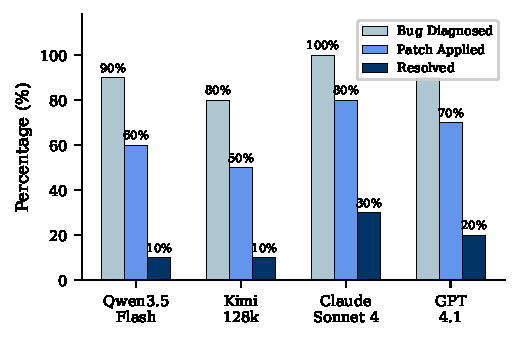
\includegraphics[width=\linewidth]{fig_results.pdf}
\caption{Evaluation results across four models in multi-turn mode ($K{=}5$). All models diagnose bugs at high rates (80\% or above), but resolve rates remain between 10\% and 30\%, revealing a persistent gap between bug comprehension and precise code editing.}
\label{fig:bar_results}
\end{figure}

\subsection{Failure Mode Analysis}

We categorize failures into four stages as shown in Table~\ref{tab:failure}. Each instance-model pair is classified by the earliest stage at which the agent fails.

\begin{table}[t]
\centering
\caption{Failure mode breakdown (multi-turn, $K{=}5$, representative subset). Each cell shows the number of instances failing at that stage.}
\label{tab:failure}
\begin{tabular}{@{}lcccc@{}}
\toprule
Failure Stage & Qwen & Kimi & Claude & GPT \\
\midrule
Bug not diagnosed     & 1 & 2 & 0 & 1 \\
Patch format error    & 3 & 3 & 1 & 1 \\
Compile failure       & 1 & 1 & 2 & 2 \\
Tests fail (incomplete fix) & 4 & 3 & 4 & 4 \\
\midrule
Resolved              & 1 & 1 & 3 & 2 \\
\bottomrule
\end{tabular}
\end{table}

The dominant failure mode across all models is incomplete fix, where the agent addresses part of the bug but misses additional dereference sites or edge cases. Patch format error is the second most common failure, particularly for Qwen and Kimi, where the model generates a correct fix idea but produces a SEARCH block that does not exactly match the source code whitespace or formatting. This finding suggests that improving patch application robustness through fuzzy matching could unlock significant gains without improving the underlying model.

\subsection{Specification-as-Skill Results}

Table~\ref{tab:ab_results} presents the A/B results for Claude Sonnet~4, the best-performing model, on the specification-as-skill evaluation subset of 50 instances.

\begin{table}[t]
\centering
\caption{Specification-as-Skill A/B results (Claude Sonnet 4, multi-turn, 50 instances). Spec-Dependent bugs require understanding protocol semantics; Generic bugs are defensive checks such as nil guards.}
\label{tab:ab_results}
\begin{tabular}{@{}lccc@{}}
\toprule
Bug Category & $-$spec & $+$spec & $\Delta$ \\
\midrule
Generic (30 instances)       & 33\% & 33\% & 0\% \\
Spec-dependent (20 instances) & 10\% & 25\% & +15\% \\
\midrule
Overall (50 instances)       & 24\% & 30\% & +6\% \\
\bottomrule
\end{tabular}
\end{table}

The results confirm our hypotheses. Specification injection provides no benefit for generic null-check bugs where the fix pattern is well-known to the model regardless of domain context. However, for specification-dependent bugs where the correct behavior is defined by a 3GPP clause, specification excerpts yield a 15\% improvement. The token overhead from specification injection averages 12\%, which is substantially lower than the average skill overhead reported in SWE-Skills-Bench~\cite{han2025sweskills}.

These findings extend the central result of SWE-Skills-Bench to the telecommunications domain: specification utility is conditional on bug type. Unlike generic coding guidelines, 3GPP specifications define the ground truth for correct behavior, making them a category of high-utility domain-matched skill for specification-dependent bugs.

% ============================================================
\section{Discussion}
% ============================================================

\subsection{Agentic Capability as the Primary Bottleneck}

The most notable finding is the gap between bug comprehension and successful resolution. In single-turn mode, Qwen3.5-Flash correctly diagnoses over 90\% of bugs, identifying the exact function, variable, and missing check, yet achieves 0\% resolve rate. Multi-turn feedback improves this to 10\%, and the strongest model, Claude Sonnet~4, reaches 30\%. This indicates that the bottleneck for telecom software engineering is not domain knowledge but rather iterative code editing capability: the ability to read, edit, compile, test, and revise in a feedback loop.

This observation aligns with findings from SWE-Bench Mobile~\cite{yao2025swebenchmobile}, which reported up to $6\times$ performance gaps across different agent frameworks using the same underlying model.

\subsection{Comparison with General-Purpose Benchmarks}

The 30\% resolve rate achieved by Claude Sonnet~4 on SWE-Bench~5G is substantially below the 40 to 50\% rates reported for similar models on SWE-Bench Verified~\cite{jimenez2024swebench}. Several factors contribute to this gap. Go requires stricter type-correct patches than Python. The 5G NF functions are deeply nested with long function signatures and complex struct types. The SEARCH/REPLACE patch mechanism demands exact string matching, penalizing models that produce minor whitespace or formatting differences compared to the original source.

\subsection{Limitations}

The current benchmark has several limitations. The majority of instances are single-NF, single-file bugs; cross-NF coordination tasks that require modifying multiple services simultaneously remain underrepresented. The dataset is drawn exclusively from free5GC; generalization to commercial 5G stacks is untested. Our multi-turn agent uses a simplified SEARCH/REPLACE mechanism, and full agentic tools such as Claude Code or Cursor with native file editing capabilities would likely achieve higher resolve rates. Finally, the statistical conclusions from the A/B experiment should be interpreted with caution given the moderate sample size.

% ============================================================
\section{Conclusion}
% ============================================================

We have introduced SWE-Bench~5G, the first benchmark for evaluating AI coding agents on 5G core network engineering tasks. The benchmark provides 210 validated instances spanning 9 Network Functions with a dual test strategy, Docker-based reproducibility, and an automated construction pipeline. Our evaluation across four LLMs reveals that agentic iteration is the primary bottleneck, with multi-turn feedback improving resolve rates from 0\% to 10 to 30\%. The specification-as-skill experiment demonstrates that 3GPP protocol excerpts provide targeted improvement on specification-dependent bugs while offering no benefit for generic defensive checks, extending the findings of SWE-Skills-Bench to the telecommunications domain. The dataset, evaluation harness, and all experimental artifacts are publicly available at \url{https://huggingface.co/datasets/tenderzada/SWEBench5G}.

\bibliographystyle{IEEEtran}
\bibliography{references}

\end{document}
